 \section{Durchführung}
\label{sec:Durchführung}
\subsection{Aufbau}
\begin{figure}
  \centering
  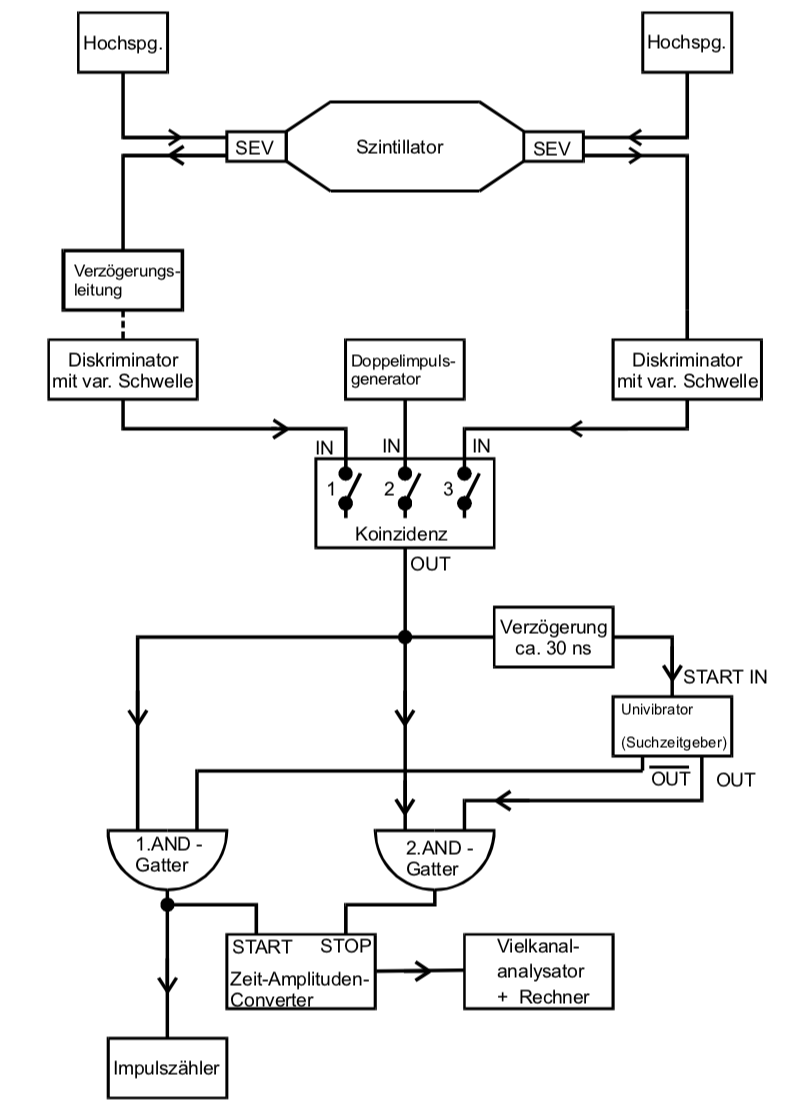
\includegraphics[width=\textwidth]{leuteBeimKacken/Schaltung.png}
  \caption{Blockschaltbild der hier genutzten Schaltung.\cite{anleitung}}
  \label{fig:Schaltung}
\end{figure}

In Abbildung \ref{fig:Schaltung} wird die Schaltung gezeigt. Im Folgenden werden die einzelnen Bestandteile von oben nach unten kurz beschrieben.

Der zentrale Detektor ist ein \SI{50}{\litre} großer Szintillationstank. Zur Aufnahme der darin erzeugten Lichtsignale und zur Übersetzung in elektrische Spannungsimpulse sind an den Enden des Tanks Photomultiplier angebracht. Diese können auch durch thermisches Rauschen ein Signal erzeugen. Um dessen Einfluss auf die Messung zu reduzieren wird eine Koinzidenzschaltung aufgebaut, die also nur ein Signal liefert, wenn in beiden SEVs gleichzeitig ein Signal auftritt. Dieses Verfahren funktioniert, weil das Rauschen der beiden SEVs unkorreliert verläuft und deshalb nur ein Myonsignal gleichzeitig in beiden SEVs ein Signal erzeugt. Ein Ausgleich der systematischen elektronischen relativen Verzögerung eines SEVs zum anderen wird durch eine Verzögerungsleitung geleistet. Eine zusätzliche Rauschunterdrückung wird durch Diskriminatoren geleistet, die Signale bis zu einer einstellbaren Schwelle nicht durchlassen. Da Rauschpulse augrund ihrer Entstehung durch einzelne Elektronen kleiner als Signalpulse sind, werden sie unterdrückt.

Der Koinzidenzschaltung folgend befindet sich die Stopuhrschaltung. Diese teilt das Signal zunächst auf je einen Eingang zweier logischer AND-Gatter sowie einen Univibrator auf. So bald nun ein Myonsignal eintritt, erhält das erste AND-Gatter sowohl von der direkten Leitung als auch von der Leitung über den Univibrator ein Signal. Damit sendet es ein Signal weiter an den später beschriebenen Zeit-Amplituden-Converter (TAC). Nach Aussendung des Signals an das erste AND-Gatter startet im Univibrator die einstellbare Suchzeit $T_\text{S}$ nach einem zweites Signal. Ein Signal das innerhalb dieser Zeit den Univibrator durchquert wird nicht an das erste dafür aber an das zweite AND-Gatter weitergeleitet. Dieses erhält also dann an beiden Eingängen ein Signal und sendet so ein Signal an den Stop-Eingang des TAC. Diese Methode kann benutzt werden, da der mittlere zeitliche Abstand von zwei einfallenden Myonen klein gegenüber ihrer Lebensdauer ist. Ein über den gesamte Zerfallszeitbereich konstanter Untergrund hat seinen Ursprung also darin dass zwei Myonen statistisch bedingt mit einem zeitlichen Abstand von $t<T_\text{S}$ in den Tank eintreten. $T_\text{S}$ sollte also so groß gewählt werden, dass möglichst viele Messwerte der Zerfallszeiten genommen werden können, aber so klein, dass der Untergrund nicht zu groß wird.
Der TAC wandelt den zeitlchen Abstand von Start- und Stop-Signal in einen dem proportional großen Spannungsimpuls um. Dieser wird an einen Vielkanalanalysator geleitet und seiner Höhe entsprechend der Zähler im entsprechenden Kanal hochgezählt. Das Histogramm der Kanäle kann im Rechner ausgelesen werden.

\subsection{Einstellen der Apparatur}
Um sich mit der Apparatur vertraut zu machen und ihre Funktionsweise zu überprüfen werden vor der eigentlichen Messung einige Tests durchgeführt.

Zunächst werden die Impulse aus den SEVs vor und nach den Diskriminatoren am Oszilloskop untersucht. Vorher sollten sie unterschiedliche Eigenschaften besitzen und danach gleich hoch und lang sein. Außerdem wird mit einem Zählwerk überprüft, ob beide Leitungen ähnliche Impulsraten aufweisen und dies mit der Schwelle am Diskriminator eingestellt. Darauf folgend wird untersucht welche Verzögerungszeit zwischen den SEVs die maximale Zählrate nach der Koinzidenzschaltung liefert. Dazu wird die Verzögerung in beide Richtungen variiert und für je zehn Sekunden die Impulszahl gemessen.
Außerdem wird die Zählrate nach der Koinzidenzschaltung mit den Zählraten der Eingänge verglichen um die Rauschunterdrückung zu überprüfen.

Als nächstes werden Univibrator und TAC justiert. Die Suchzeit des Univibrators wird etwas größer eingestellt als der Zeitmessbereich des TAC. Mit Hilfe eines Doppelimpulsgenerators wird überprüft ob der TAC korrekt arbeitet, also Spannungsimpulse liefert dessen Höhe proportional zum zeitlchen Abstand der Impulse ist. Dies wird am PC mit Vielkanalanalysator kontrollliert. So wird auch eine Zeiteichung durchgeführt, da man den eingestellten Abstand der Impulse so einem Kanal zuordnen kann.

Um abzuschätzen wie oft Myonen detektiert werden, also auch die die nicht im Behälter zerfallen, wird noch an das erste AND-Gatter ein Zählwerk angeschlossen. Mit diesem Wert kann zusammen mit der Messzeit der Untergrund bestimmt werden.

Dann kann mit der eigentlichen Messung begonnen werden, bei der die individuellen Lebensdauern \num{20} bis \num{30} Stunden aufgenommen werden und als Histogramm dargestellt werden. Dann kann mit der in Kapitel \ref{sec:Lebensdauerbestimmung} beschriebenen Methode die mittlere Lebensdauer bestimmt werden.
